% (c) 2014 Dimitrios Vrettos - d.vrettos@gmail.com
% (c) 2014 Claudio.carboncinii - claudio.carboncini@gmail.com
% (c) 2014 Daniele Zambelli - daniele.zambelli@gmail.com

\section{La leggenda di Pitagora e la scoperta di un numero inquietante}

La vita e l'opera di Pitagora hanno costituito oggetto
di approfondite ricerche da parte degli storici di tutti i tempi.
Nonostante le indagini più accurate, i fatti della vita di Pitagora
realmente accertati sono veramente pochi. Si dice sia nato a Samo 
nel~572~\aC\footnote{O nel~575~\aC\ per altri autori.} dove vi regnava il 
tiranno Policrate; non sopportando la tirannia, si trasferì in Egitto con 
un incarico di lavoro presso il faraone Amasi. Sembra che poi abbia
viaggiato in Babilonia prima di approdare a Crotone dove fondò una
Scuola che accolse numerosi discepoli. Pitagora propose un sistema
matematico della natura: la spiegazione dei fenomeni naturali doveva
avvenire attraverso la ricerca di relazioni tra numeri. Pensava che
tutti i corpi fossero formati da punti materiali o monadi combinate in
modo da formare le varie figure geometriche e il numero totale di tali
unità rappresentava l'oggetto materiale. Da qui
nasceva la dottrina secondo la quale tutte le cose che si conoscono
hanno un numero; senza questo nulla sarebbe possibile pensare, né
conoscere; la spiegazione dei fenomeni naturali può essere raggiunta
solo attraverso l'aritmetica.

Per i pitagorici esistono due soli tipi di numeri: gli interi e le
frazioni. Ogni numero aveva sia una rappresentazione simbolica che un
significato simbolico: il numero~5 veniva assunto a rappresentare il
matrimonio, essendo la somma del primo numero dispari, il~3, con il
primo numero pari, il~2.

Fu dunque terribile la scoperta di un nuovo tipo di numero che non è
né intero né frazionario, questo numero si ottiene calcolando per
mezzo del teorema di Pitagora la misura della diagonale di un quadrato
di lato uno. Questo nuovo numero, che oggi scriviamo~$\sqrt{2}$, non
poteva essere espresso in nessun modo come frazione, cioè rapporto di
numeri interi. Ad esso i pitagorici diedero il nome di
\emph{arreton}, cioè indicibile, inesprimibile. La scoperta fu
mantenuta segreta. La leggenda narra che Ippaso, discepolo della
Scuola, morì affogato perché violò il giuramento che aveva fatto
di non diffondere questa terribile verità.

Oggi questi numeri li chiamiamo \emph{numeri irrazionali}, termine che
riflette la stessa idea di inesprimibilità attribuita loro dai
pitagorici \footnote{Per approfondire l'argomento: G. Masini, \textit{Storia
della matematica}, SEI; John D. Barrow, \textit{La luna nel pozzo
cosmico}, CDE; Ludovico Geymonat, \textit{Storia del pensiero
filosofico e scientifico}, Garzanti, vol.~1; David Bergamini e redattori
di Life, \textit{La matematica}, Mondadori; Morris Kline,
\textit{Matematica la perdita della certezza}, A. Mondadori.}.

\section{I numeri irrazionali}
Applicando il teorema di Pitagora a un quadrato di lato unitario per
calcolare la misura della diagonale i pitagorici individuarono un nuovo
tipo di numero, oggi indicato con~$\sqrt{2}$.

Fissiamo sulla retta orientata~$r$ l'unità di misura e disegniamo il quadrato 
di lato~1. Ci proponiamo di calcolare la misura della sua diagonale~$OB$.

\begin{center}
 % (c) 2013 Claudio Carboncini - claudio.carboncini@gmail.com
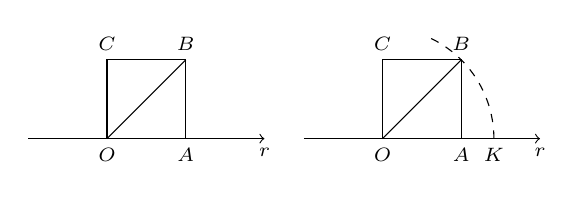
\begin{tikzpicture}[x=10mm, y=10mm, font=\scriptsize]
  \draw [->] (0,0) -- (3,0) node [below] () {$r$};
  \draw (1,0) rectangle (2,1);
  \draw (1,0) -- (2,1);

  \coordinate[label=below:$O$] (O) at (1,0);
  \coordinate[label=below:$A$] (A) at (2,0);
  \coordinate[label=above:$C$] (C) at (1,1);
  \coordinate[label=above:$B$] (B) at (2,1);

  \begin{scope}[xshift=35mm]
    \draw [->] (0,0) -- (3,0) node [below] () {$r$};
    \draw (1,0) rectangle (2,1);
    \draw (1,0) -- (2,1);

    \coordinate[label=below:$O$] (O) at (1,0);
    \coordinate[label=below:$A$] (A) at (2,0);
    \coordinate[label=above:$C$] (C) at (1,1);
    \coordinate[label=above:$B$] (B) at (2,1);
    \coordinate[label=below:$K$] (K) at (2.414,0);

    \draw[dashed] (2.414,0) arc [start angle=0, end angle=65,radius=1.414cm,];

  \end{scope}
\end{tikzpicture}

\end{center}

Il triangolo~$OAB$ è retto in~$A$, quindi per il teorema di
Pitagora~$\overline{OB}^{2}=\overline{OA}^{2}+\overline{AB}^{2}$.
Sostituiamo le misure:~$\overline{OB}^{2}=1^2+1^2=2$. 
Per ottenere~$\overline{OB}$
dobbiamo estrarre la radice quadrata e quindi~$\overline{OB}=\sqrt{2}$.

Sappiamo che `estrarre la radice quadrata' di un numero significa trovare 
quel numero che elevato al quadrato dà~2. Questo numero deve esistere, 
nel senso che esiste un punto sulla retta~$r$ che lo rappresenta, 
per costruirlo graficamente si può tracciare l'arco di circonferenza di 
centro~$O$ e raggio~$OB$ e determinando su $r$ il punto~$K$ estremo 
del segmento con~$OK = OB$.

Dalla posizione del punto~$K$ possiamo dire che~$1<\sqrt{2}<2$. Il
valore cercato evidentemente non è un numero intero. Può essere un
numero decimale finito? Compiliamo una tabella che contenga nella prima
riga i numeri con una sola cifra decimale compresi tra~1 e~2 e nella
seconda riga i rispettivi quadrati:

\begin{center}
\begin{tabular}{ccccccc}
\toprule
$x$ & 1,1 & 1,2 & 1,3 & 1,4 & 1,5 & 1,6\\
$x^{2}$ & 1,21 & 1,44 & 1,69 & 1,96 & 2,25 & 2,89\\
\bottomrule
\end{tabular}
\end{center}

Osserviamo che il numero~2 è compreso tra~$1,4^{2}$ e~$1,5^{2}$,
di conseguenza~$1,4<\sqrt{2}<1,5$, ma ancora
non possiamo precisare il suo valore, anche se abbiamo ristretto
l'intervallo in cui si trova il punto~$K$. Diciamo che~1,4 è un valore 
approssimato per difetto di~$\sqrt{2}$ mentre~1,5
è un valore approssimato per eccesso; scrivendo~$\sqrt{2}=1,4$
oppure~$\sqrt{2}=1,5$ commettiamo un errore minore di~1/10.

Per migliorare l'approssimazione e tentare di ottenere~$\sqrt{2}$
come numero razionale costruiamo la tabella dei numeri
decimali con due cifre compresi tra~1,4 e~1,5:

\begin{center}
\begin{tabular}{ccccc}
\toprule
$x$ &1,41 &1,42 &1,43 &1,44\\
$x^{2}$ & 1,9881 & 2,0164 & 2,0049 & 2,0776\\
\bottomrule
\end{tabular}
\end{center}

Ora possiamo dire che~1,41 è un valore approssimato per difetto di~$\sqrt{2}$ 
mentre~1,42 è un valore approssimato per eccesso, con un errore 
dell'ordine di~1/100. Abbiamo quindi migliorato l'approssimazione e di 
conseguenza abbiamo ristretto l'intervallo in cui cade il punto~$K$. 
Ma ancora non abbiamo trovato un numero razionale che sia uguale a~$\sqrt{2}$.

Continuando con lo stesso procedimento costruiamo due classi di numeri 
razionali che approssimano una per difetto e una per eccesso il numero 
cercato, restringendo ogni volta l'ampiezza dell'intervallo in cui cade 
il punto~$K$.
Il procedimento continua all'infinito e le cifre decimali che troviamo non 
si ripetono periodicamente.

\begin{center}
 \begin{tabular}{lcll}
\toprule
Valore per difetto & Numero &Valore per eccesso & Ordine dell'errore\\
\midrule
1	& $\sqrt{2}$ 	& 2 	&1\\
1,4	& $\sqrt{2}$	&1,5 	& $10^{-1}$\\
1,41	& $\sqrt{2}$	& 1,42	& $10^{-2}$\\
1,414	& $\sqrt{2}$	&1,415	&$10^{-3}$\\
1,4142	& $\sqrt{2}$	& 1,4143&$10^{-4}$\\
\ldots	& $\sqrt{2}$	&\ldots	&\ldots\\
\bottomrule
\end{tabular}
\end{center}

Per arrivare a concludere che~$\sqrt{2}$ non è un numero razionale,
possiamo ragionare nel seguente modo. Supponiamo per assurdo che~$\sqrt{2}$
sia un numero razionale e precisamente~$\sqrt{2}=\frac{a}{b}$ con~$a$ e~$b$ 
primi tra loro; si avrebbe, elevando al quadrato, $2=\frac{a^{2}}{b^{2}}$.

Se si eleva un numero al quadrato significa elevare al quadrato le
singole potenze dei fattori primi in cui questo si scompone. I fattori
primi di~$a^{2}$ e di~$b^{2}$ sono gli stessi di~$a$ e di~$b$ con
gli esponenti raddoppiati. Quindi anche~$a^{2}$ e~$b^{2}$
sono primi tra di loro e~$a^{2}$ non può essere il doppio di~$b^{2}$.
Se lo fosse dovrebbe essere almeno il quadruplo. 
Quindi~$2\ne\frac{a^{2}}{b^{2}}$ e~$\sqrt{2}\ne\frac{a}{b}$.

Oltre a~$\sqrt{2}$ vi sono altri infiniti numeri che non possono
essere scritti come frazione. Per esempio tutte le radici quadrate di
numeri naturali che non sono quadrati perfetti e tutte le radici
quadrate di frazioni che non sono il quadrato di alcuna frazione.

Le radici quadrate dei numeri che non sono quadrati perfetti e che non
sono il quadrato di alcuna frazione sono numeri decimali con infinite 
cifre decimali non periodiche; essi perciò possono essere scritti
solo in maniera approssimata. Questi numeri sono detti 
\emph{numeri irrazionali} e insieme ad altri, che conoscerete
in seguito, costituiscono l'insieme~$\insJ$ dei numeri irrazionali.
